\subsection{Voorbeelden}

\emph{Voorbeelden}

\noindent \uline{Voorbeeld 1}: bespreek de functie $f$ met voorschrift $f(x)=\sqrt{10-2x}-2$.

\begin{figure}[h]
	\centering{}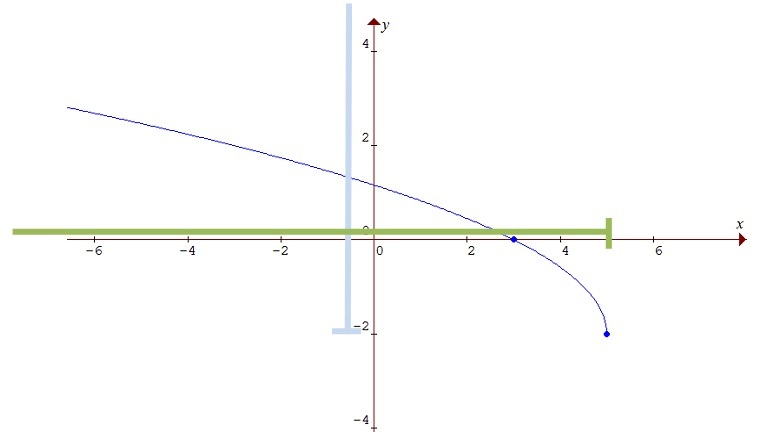
\includegraphics[height=5cm]{2_elem_rekenvaardigheden_B/inputs/reeel_vb1.jpg} 
\end{figure}


\noindent \textbf{Domein}: de uitdrukking onder de vierkantswortel
mag niet negatief worden:

\noindent 
\begin{eqnarray*}
	\begin{array}{cccc}
		& 10-2x & \geqslant & 0\\
		\iff & 10 & \geqslant & 2x\\
		\iff & 5 & \geqslant & x\\
		\iff & x & \leqslant & 5
	\end{array}
\end{eqnarray*}


\noindent Besluit: voor $x$ zijn alle waarden van $-\infty$ tot
en met $5$ toegelaten. We schrijven: $\textrm{dom}\:y=]-\infty,5]$ 

\medskip{}


\noindent \textbf{Beeld}: de kleinste functiewaarde wordt
bekomen als de wortel $0$ is. Vierkantwortels geven altijd een positief
resultaat (of nul). De uitdrukking onder de wortel wordt $0$ als
$x=5$. We zien dat $f(5)=-2$. Er is geen bovengrens, dus het bereik
loopt tot $+\infty$.

\noindent Besluit: $\textrm{bld}f=[-2,+\infty[$

\medskip{}


\noindent \textbf{Nulpunten}: voor welke waarden van $x$ wordt $f(x)=0$?

\noindent 
\begin{eqnarray*}
	\begin{array}{cccc}
		& \sqrt{10-2x}-2 & = & 0\\
		\iff & \sqrt{10-2x} & = & 2\\
		\iff & \left(\sqrt{10-2x}\right)^{2} & = & 2^{2}\\
		\iff & 10-2x & = & 4\\
		\iff & 6 & = & 2x\\
		\iff & x & = & 3
	\end{array}
\end{eqnarray*}


\noindent Besluit: er is slechts 1 nulwaarde, en dit is $x=3$ .

\medskip{}


\noindent \textbf{Symmetrie}: we gaan na of het beeld van $-x$ hetzelfde
of het tegengestelde resultaat geeft als de gegeven functie. $f(-x)=\sqrt{10-2(-x)}-2=\sqrt{10+2x}-2$.
Dit is noch gelijk aan $f(x)$ noch gelijk aan $-f(x)$. Deze functie
is dus noch even, noch oneven.

\noindent \bigskip{}


\noindent \uline{Voorbeeld 2}: bespreek de functie met voorschrift $f(x)=\frac{1}{x-2}$.

\begin{figure}[h]
	\centering{}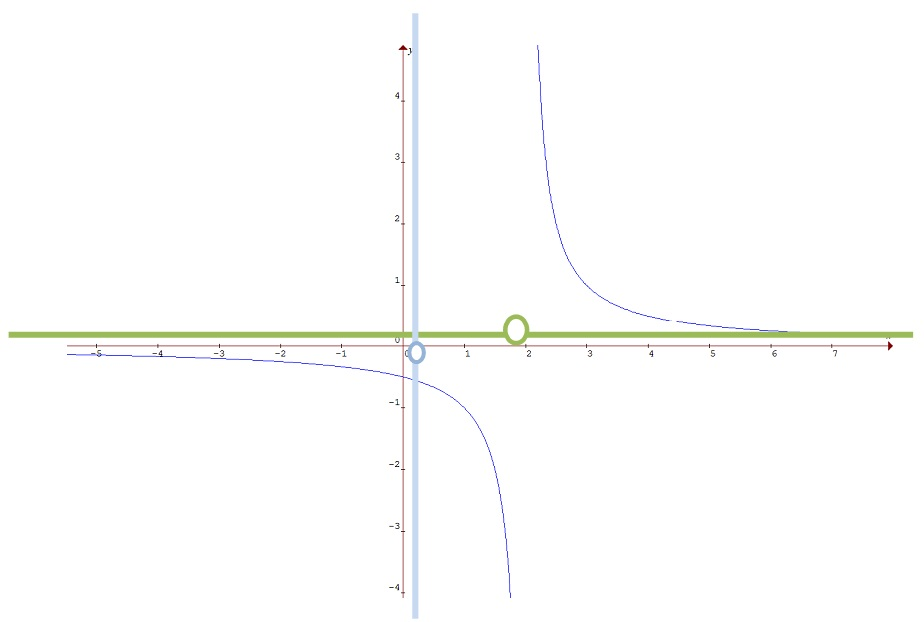
\includegraphics[height=5cm]{2_elem_rekenvaardigheden_B/inputs/reeel_vb2.jpg} 
\end{figure}


\noindent \textbf{Domein}: de noemer mag niet nul worden (omdat een
getal delen door $0$ geen getal $\in \mathbb{R}$ is):

\noindent 
\begin{eqnarray*}
	\begin{array}{cccc}
		& x-2 & \neq & 0\\
		\iff & x & \neq & 2
	\end{array}
\end{eqnarray*}


\noindent Besluit: $\textrm{dom}\:y=\mathbb{R}\setminus\{2\}$ 

\medskip{}


\noindent \textbf{Beeld}: er is geen bovengrens en geen ondergrens,
maar de breuk zal echter nooit $0$ worden.

\noindent Besluit: $\textrm{bld}f=\mathbb{R}_{0}$

\medskip{}


\noindent \textbf{Nulpunten}: aangezien een breuk enkel nul kan worden
als de teller nul is, zal dit bij deze functie nooit gebeuren. Er
is dus geen snijpunt met de $x$-as.

\noindent Besluit: deze functie heeft geen nulpunten.

\medskip{}


\noindent \textbf{Symmetrie}: we gaan na of het beeld van $-x$ hetzelfde
of het tegengestelde resultaat geeft als de gegeven functie. $f(-x)=\frac{1}{(-x)-2}=-\frac{1}{x+2}$.
Dit is noch gelijk aan $f(x)$ noch gelijk aan $-f(x)$. Deze functie
is dus noch even, noch oneven.

\noindent \bigskip{}


\noindent \uline{Voorbeeld 3}: bespreek de sinusfunctie $f(x)=\sin(x)$ 

\begin{figure}[h]
	\centering{}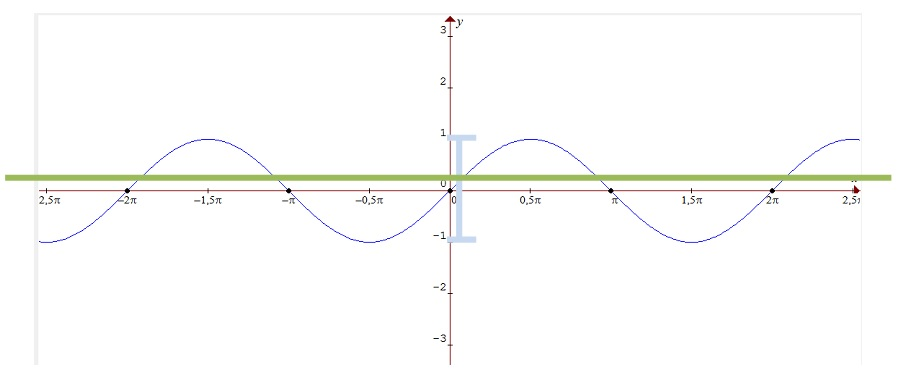
\includegraphics[height=5cm]{2_elem_rekenvaardigheden_B/inputs/reeel_vb3.jpg} 
\end{figure}


\noindent \textbf{Domein}: we mogen op de plaats van $x$ gelijk welke
hoek invullen, de sinus zal steeds bestaan.

\noindent Besluit: $\textrm{dom}\:y=\mathbb{R}$ 

\medskip{}


\noindent \textbf{Beeld}: we lezen op de $y$-as het beeld af. De
functiewaarden voor de sinus kunnen nooit groter zijn dan $1$ of
kleiner dan $-1$

\noindent Besluit: $\textrm{bld}f=[-1,1]$

\medskip{}


\noindent \textbf{Nulpunten}: de $x$-as wordt gesneden als $\sin(x)=0$.
Dit gebeurt zowel voor $x$-waarden gelijk aan $\{0,\pi,2\pi,3\pi,...\}$
als ook voor $\{...,-3\pi,-2\pi,-\pi,0\}$

\noindent Besluit: de snijpunten met de $x$-as zijn de punten $\{...,(-2\pi,0),(-\pi,0),(0,0),(\pi,0),(2\pi,0),...\}$
of iets korter genoteerd als: $\{(k\pi,0)\:\textrm{met}\:k\in\mathbb{Z}\}$

\medskip{}


\noindent \textbf{Symmetrie}: via de goniometrische formules vinden
we snel dat $f(-x)=\sin(-x)=-\sin(x)=-f(x)$ , dus kunnen we zeggen
dat deze functie oneven is (symmetrisch t.o.v. de oorsprong).
